\section{Conception of adaptive measurements}\label{sec:concept}
\subsection{Estimation of parameters}
In wide class of the experiments the main goal can be described as follows: we have ``black box'' with some output that we can measure, and the idea is to get information about parameters of this ``black box'' using only this output signal. The problem is that we have some noises acting on our system. The procedure of estimation of the parameters from noisy signal is called filtering. To specify the problem, let's take a look of Fig.\ref{pic:stfilt},where we have some dynamical system with output signal $x(t)$ (this value can be a vector). We proceed measurements and have some data $y(t)$; then use filter and get some estimated value $\tilde{x}(t)$. 
The choice of filtering procedure depends on the particular problem. Most common filters minimize error or mean square error, but there are plenty of other.  
We call optimal the filter that achieves best estimation. 
% This approach is part of the control and estimation theory \cite{Slotine1991} and has lot of applications, particularly it can be used in quantum measurements \cite{Wiseman2011a}.
\subsection{Adaptive filtering}

\begin{figure}
\vspace{-5ex}
\begin{minipage}{0.6\linewidth}
\includegraphics[width=1\linewidth]{meas_dia.pdf}
\caption{Classical filtering problem}
\label{pic:stfilt}
\end{minipage}
\hfill
\begin{minipage}[h]{0.4\linewidth}
\includegraphics[width=1\textwidth]{AdaptiveFilter_C.png}
\caption{\footnotesize Block-scheme of the adaptive filter. Here $x(n)$ is signal, $\tilde{d}(n)$ is estimation of desired signal $d(n)$ and $e(n)$ is error.}
\label{pic:ad1}
\end{minipage}
\end{figure}

One of the way of solving filtering problem is so-called adaptive filtering. Adaptive filter adjusts its filtering function using error signal in order to achieve optimal filtering \cite{Farhang-Boroujeny1998,Sastry1989,Haykin2003,Drumright1998,Nationale1991,Huzmezan2002}.
Classic adaptive filter has quite simple scheme: as illustrated in Fig. \ref{pic:ad1}, we estimate the output signal in order to reach desired value. On the each step we use an error between estimated signal an desired to change the adaptive filter.
\\
But in the quantum case there are significant differences: the most important is presence of uncertainty principle, so we can not measure, for example, two different optical quadratures (or position and momentum) with any precision. Also we can not disturb the signal from system before measurement, otherwise we loose information about the state of the system.
That is why we have to modify existing schemes for quantum case.
We propose the following scheme for quantum case as shown in Fig. \ref{pic:quantad}\\

The procedure of such filtering is the following:
\begin{enumerate}
 \item $x(t)$ is a signal from the system, we measure it and get $\tilde{y}(t)$, then filter it in order to get estemation $\tilde{x}(t)$
 \item We use this estimation as initial state for the second stage. During this stage our initial state evolves and then we measure it and get second estimation $\tilde{\tilde{y}}(t+\varDelta t)$
 \item We make measurements at the time $t+\varDelta t$ and get approximation $\tilde{y}(t+\varDelta t)$
 \item Calculating error $\varepsilon(t+\varDelta t) = \tilde{\tilde{y}}(t+\varDelta t) - \tilde{y}(t+\varDelta t)$  and using errors in previous moments we can predict the optimal filter at time $t+2 \varDelta t$
 \item Now we can change this filter according to our prediction
\end{enumerate}

So, at each step of our measurement procedure we do the following stages of optimal quantum measurements: preparation(``create'' the state $\tilde{x}$)\cite{Rehbein2009m}, evolution(wait some small time $\varDelta t$) and verification(the second approximation and optimization of the filter)\cite{Miao}

\begin{figure}[!]
\begin{center}
 \includegraphics[width=1\linewidth]{adapt_1.pdf}
 \caption{Adaptive filter for quantum measurements}
\label{pic:quantad}
\end{center}
\end{figure}
In spite of the fact that classical case and quantum one have lots of differences, both of them can be described by similar equations,well known from control theory.
% \subsection{Application}
% This idea can be easily applied to our particular case of GW detection. We consider the usual interferometer with homodyne detection, but we change the homodyne angle in that way to minimize the cost function for next measurement. Such scheme would be adaptive and probably can help us to deal with some specific tasks. We shall discuss it later.

\begin{figure}
\begin{minipage}[b]{0.6\linewidth}
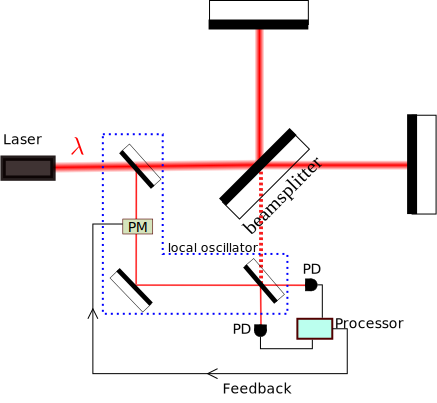
\includegraphics[width=1\textwidth]{ad_m.png}
\caption{Scheme of adative measurements for interferometer}
\end{minipage}
\hspace{0.1\linewidth}
\begin{minipage}[b]{0.3\linewidth}
 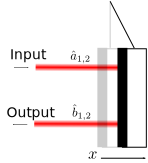
\includegraphics[width=1.0\textwidth]{system}
 \caption{Model of the system}
 \label{pic:sys}
\end{minipage}

\end{figure}
\subsection{Previous researches}
Due to the clearness of the idea, adaptive measurements are extremely popular in classical experiments. There are some fields of application, such as noise cancelling, seismic data processing,beamforming, \textit{etc.} \cite{Farhang-Boroujeny1998}
Currently the quantum adaptive control is a fast developing field \cite{Wiseman2011a,Ahn2008}, and some of the works were devoted to the adaptive filtering.
The main idea of adaptive quantum measurement was proposed almost at the same time at different scientific groups \cite{Wiseman1997,Braginsky1993}.The significant contribution was made by Wiseman and Berry is series of papers on adaptive measurements of phase of the light \cite{Berry2008,Berry2001,Berry2002,Measurements1995m}
By the moment there are a few works on the adaptive measurements in GW detectors \cite{Hentschel2010,Dhurandhar2008}.

In my work I investigate some new ideas: firstly I consider a new scheme for adaptive measurements and general method for solving such tasks, secondly, I consider the case of opto-mechanical system (not just optical, as in previous works), and thirdly, I provide some real estimation for LIGO experiment in order to make a decision if such an approach could be feasible to realize.
